\chapter{PP：\emph{依赖类型}的表格打印器}
本文倡导依赖类型编程实践，而最好的倡导方式就是讲解实例。各种实例中，又以
那些具有工程价值，被实际运用于项目中的为贵。因而，我们专门用一章来介绍 \Tigris 实践中使用的
依赖类型编程，以此作为范例，并承上启下，令读者熟悉何为依赖类型，为下一部分的定理证明子系统 \Tigrisd 叙述奠基。

实际上，\Tigris 使用的依赖类型完全不止本节的标题，还包括一些（互）递归函数的停机证明，但下文
以叙述 PP 打印器的设计与实现为主，并以此展示依赖类型论如何能帮我们在编译期发现更多的程序错误，
并为读者提供依赖类型方法论的基本认识。

PP 打印器自身，被广泛运用于命令行信息的\emph{美观输出}，例如
\Tigris 的 REPL 可以通过 \texttt{\#check} 命令打印类型环境表格；编译器 CLI 前端则可通过
\texttt{-h, --help} 参数打印帮助信息表格。

\begin{analysis}
  表格，本质上来说无非是一\emph{矩阵}。各种表格因为其承载数据的不同，即\emph{表头}的不同而不同。例如，
  表头（姓名、性别、年龄）显然和表头（产品名称、制造商、序列号、定价）指代的表格在意义上不同。然而，
  我们如何在语言中自然的区分两者——一种想法是利用类型检查器，只要能够区分两种表格的\emph{类型}即可，
  因此，我们转向依赖类型论的支持，PP 打印器由此而生。

  考虑作为 \texttt{List}（列表）的表头，可将其变换为\emph{动态长度}的元组，即
  使元组类型\emph{依赖于}表头长。这样，我们就要求该元组的类型与长度必须与表头一致，
  才能通过类型检查器。
\end{analysis}
由此，我们可以定义
\begin{minted}[numbers=left,frame=single]{lean4}
abbrev ToProd (as : List α) (m : Type -> Type) : Type :=
  match as with
  | [] => PUnit
  | [_] => mα
  | _ :: x :: xs => m α × ToProd (x :: xs) m
abbrev Row := ToProd header id
\end{minted}
%\begin{figure}[H]
%  \begin{subfigure}[c]{0.5\textwidth}
%  \end{subfigure}%
%  \begin{subfigure}[c]{0.5\textwidth}
%    \begin{align*}
%      &\mathsf{ToProd}\ (as : \mathsf{List}\ \alpha)\ (m : \mathbf{Type}\to\mathbf{Type}) =\\
%      &\quad
%      \begin{cases}
%        \mathsf{PUnit} &as = [];\\
%        m\ \alpha &as = [x];\\
%        m\ \alpha \times \mathsf{ToProd}\ (x :: xs)\ m &as = \cdot :: x :: xs.
%      \end{cases}\\
%      &\mathsf{Row}\ \textit{h} = \mathsf{ToProd}\ \textit{h}\ \mathrm{id}_\mathbf{Type}.
%    \end{align*}
%  \end{subfigure}
%  \caption{\texttt{ToProd} 在 Lean 中与数学中的定义比较}
%\end{figure}

上述定义可以理解为，$\mathsf{ToProd}\ (as : \mathsf{List}\ \alpha)\ f$ 可\emph{消去到} 1) $\mathsf{PUnit}$
泛类型宇宙的幺元 2) $f\ \alpha$ 或 3) $f\ \alpha \times \mathsf{ToProd}\ (\mathsf{cdr}\ as)\ f$，
根据 $as$ 的形状 1) 为空；2) 为单个类型；3) 包含两个及以上的类型。定理证明器术语中，称像这样
在\underline{项上做模式匹配并消去到\emph{不定}类型}的操作为 large elimination.

也就是说，\texttt{ToProd} 类型构造子（在此可看作类型上的函数）可以根据
$as$ 的\emph{值}（长度）\footnote{
准确地说，是 $2 + n$ 个类型之一，对长度为 $n$ 的 $as$.
}，消去到上述三个类型之一。可以发现，虽然我们是通过模式匹配实现这一变换的，
但为了和值上的编程做区分，称这种思考方式为基于\emph{消去子}（eliminator/recursor）的解读，且
该模式匹配在 Lean 的内核中也确实以消去子应用的形式存在。

\begin{remark}[motive]
\emph{Motive}（动机，定义中是 $m$）是类型论术语，表示消去的目标类型（或其一部分），可以理解为
函数式编程在数据结构中常用的 \texttt{map} 函数。而 \mintinline{lean4}{abbrev} 比起 \mintinline{lean4}{def}
又可保证上述定义是\emph{可消去的}（reducible），而非\emph{半消去}或\emph{不可消去}，这使得 Lean 的类型检查器
能够自动按需查看上述定义。
\end{remark}

\paragraph{表格行的定义} 现在规定，表格的一行（\texttt{Row}）由 \texttt{ToProd header id} 编码。这样，我们保证
某一表格必须与其表头的格式（形状）一致，保证不同表格可以根据表头区分，否则产生
类型检查器将报错。在此基础上，我们又可定义表格类型 \mintinline{lean4}{abbrev TableOf := Array (Row header)}.

注意，上述定义的类型 \texttt{Row}、\texttt{TableOf} 都是类型构造子，需要表头（\texttt{header}）作为参数传入。
之所以使用连续数组 \texttt{Array} 而非列表（链表）\texttt{List}，是因为前者性能更好。此外，虽然表格的列数由
表头固定，但表格的行数（条目数）显然是可以自由增长的，因而此处用动态数组编码是恰当的。

作为用户，表格打印器最重要的需求是\emph{美观}，最少也应当\emph{看起来像一个表格}。定义
\begin{minted}[numbers=left,frame=single]{lean4}
inductive Alignment | left | center | right
inductive PadsBy | perCell | perCol
abbrev Align := ToProd header λ _ => Alignment
abbrev OverrideWidth := ToProd header λ _ => Option Nat
\end{minted}
\texttt{Align} 和表头形状相同，表示每一列的对齐格式（左对齐、居中、右对齐）；
\texttt{PadsBy} 表示空白填充（padding）策略。\texttt{perCell} 要求所有格子具有相同宽度，且
该宽度由最大的格子决定；\texttt{perCol} 则与之类似，但单独为\emph{每列}按照其最大的格子设置宽度；
\texttt{OverrideWidth} 则能够给用户以细粒度的格子宽度控制，允许用户手动、独立设置每一列的
宽度。

除此之外，我们还定义了格子两侧的留白（margin）长度、截断开关，后者用于在输出时跳过零长度的格子。听起来很简单，
但使用恰当时能产生意想不到的作用，比如图 \ref{pp:comp} 通过结合两者实现缩进功能，用于打印编译器前端的帮助信息。
\begin{figure}[h]\centering
\begin{subfigure}{0.35\textwidth}\centering
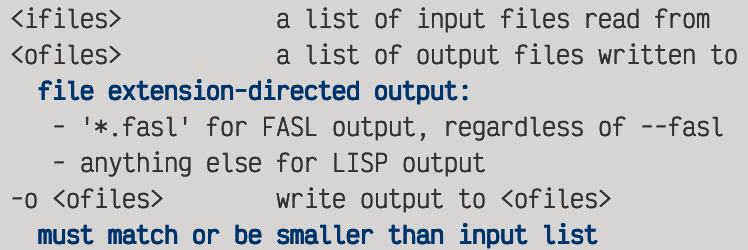
\includegraphics[width=\textwidth]{assets/term2}
\end{subfigure}%
\begin{subfigure}{0.65\textwidth}\centering
    \begin{minted}{lean4}
(.str "<ofiles>", .str "a list of input files read from")
(.str "", .byl "file extension-directed output:")
(.str "", .str " - '*.fasl' for FASL output ..")
(.str "", .str " - anything else for LIPS output")
    \end{minted}
\end{subfigure}
\caption{表格打印器的输出与对应的源代码条目}\label{pp:comp}
\end{figure}
\begin{figure}[htb]
\centering
%\begin{subfigure}{0.55\textwidth}\centering
%\begin{minted}{lean4}
%def ovTostr (ov : OverrideWidth header)
%  : String :=
%  match header with
%  | [] => "" | [_] => toString ov
%  | %[_, _ | _] =>
%    toString ov.1 ++ ovTostr ov.2
%\end{minted}
%\end{subfigure}%
%\begin{subfigure}{0.5\textwidth}\centering
%\begin{minted}{lean4}
%def zeroOverride (header : List Text.SString)
%  : OverrideWidth header :=
%  match header with
%  | [] => () | [_] => none
%  | %[_, y | ys] =>
%    (none, zeroOverride (y :: ys))
%\end{minted}
%\end{subfigure}\vspace{1em}
\begin{subfigure}{0.55\textwidth}\centering
\begin{minted}{lean4}
def maxN (h₁ h₂ : OverrideWidth header)
  : OverrideWidth header :=
  match header with
  | [] => () | [_] => max h₁ h₂
  | %[_, _ | _] =>
    (max h₁.1 h₂.1, maxN h₁.2 h₂.2)
\end{minted}
\end{subfigure}%
\begin{subfigure}{0.5\textwidth}\centering
\begin{minted}{lean4}
def merge (h₁ h₂ : OverrideWidth header)
  : OverrideWidth header :=
  match header with
  | [] => () | [_] => max h₁ h₂
  | %[_, _ | _] =>
    (h₂.1 <|> h₁.1, merge h₁.2 h₂.2)
\end{minted}
\end{subfigure}\vspace{.5em}
\begin{subfigure}{\textwidth}\centering
%instance : ToString $ OverrideWidth header := ⟨ovTostr⟩
%instance : Zero     $ OverrideWidth header := ⟨zeroOverride header⟩
\begin{minted}{lean4}
instance : Max      $ OverrideWidth header := ⟨maxN⟩
instance : Union    $ OverrideWidth header := ⟨merge⟩
\end{minted}
\end{subfigure}
\caption{用于计算列宽的辅助函数及对应类型类实现}\label{code:pp-col}
\end{figure}

{\setlength{\parskip}{-1em}\paragraph{Discriminant Refinement} 基于这些类型定义，图 \ref{code:pp-col} 实现了一些辅助函数。我们以这些函数为引子，引入一个在后续的 \Tigrisd，或任何
依赖类型论语言中都十分重要的机制：\emph{被匹配对象的精练}（discriminant refinement）\footnote{
精练（refine）一词是类型论术语，指通过（用户提供的）类型环境内的信息，将一个\emph{较泛}的类型
中的一部分，或整体，变为更加具体的项的过程。
}。\texttt{ToProd}，
某种意义上可以看作一个“多态”的类型（长度不同，依赖表头形状）——但无论如何，其在同一时刻只能具有一个值（类型），
因为 Lean 是静态类型语言。那么，如何告诉编译器 \texttt{ToProd} 在\underline{何时具有何种类型}呢——我们就需要通过精练
被匹配对象来实现这点了。}

精练被匹配对象是类型论术语，其含义即为字面义，指模式矩阵可以用来精练（补充）被匹配对象的
类型信息。例如，\mintinline{lean4}{match h : x with | 0 => ...} 告诉编译器 \texttt{x} 在
模式矩阵的第一个分支下\underline{一定等于 0}（而不仅仅是 $x$ 具有类型 $\mathsf{Int}$），
并在类型环境中添加一条\emph{假设}（assumption）$h : x = 0$ 以供用户使用之——根据模式匹配的语义
这显然是正确的。这一技巧在依赖类型编程中极为常见，例如在此处我们通过三个分支\emph{指导}编译器 \texttt{ToProd} 应该
具有的具体形状：
\begin{enumerate}\itemsep0em
\item 模式 \texttt{[]} 指出 $\textit{header} = []$，根据定义，\texttt{ToProd} 只能是 $\mathsf{PUnit}$；
\item 模式 \texttt{[\_]} 指出 $\textit{header} = [\cdot]$，匹配单元素（类型为 $\alpha$）。由定义 \texttt{ToProd} 只能是 $f\ \alpha$；
\item 模式 \texttt{\%[\_, \_ | \_]}，是 \texttt{\_ :: \_ :: \_} 的语法糖，指出
$\textit{header} = \cdot :: (\cdot :: \cdot)$，匹配两个及以上元素。由定义 \texttt{ToProd} 只能是“动态”长度的元组。
\end{enumerate}

从前文模式匹配“是用于解构数据结构”的解读看来，这里的模式匹配毫无用处；这是因为此处的重点在于使用模式匹配进行\emph{分情况讨论}，
告诉类型检查器额外的信息，因为其自身没有能力（类型推断做不到）分三种情况进行讨论。如果删去模式匹配，
则会产生类型检查错误，因为 Lean 自身无法推断类型，且从证明的角度考虑，不分三种情况讨论也没有办法确定 \texttt{ToProd} 的具体类型。
上面的叙述看起来复杂，但其思想很简单：任何一个接触过中学数学，学习过分情况讨论的用户，其实都已熟悉一定程度上的依赖类型编程。读者只需知道
函数定义需要\emph{照抄}类型定义的形式（三种情况）即可。

\begin{remark}[Discriminant Refinement 的常见用途]
除上述用途之外，Discriminant Refinement 最为常见的用途就是向类型环境（证明环境）中
添加条件/假设。例如，列表上的 \texttt{foldr1} 通常不允许空列表，在 Haskell 中
将之应用于空列表会出现运行时错误。然而，在依赖类型编程语言中，如 Lean，我们只需
将这一要求作为条件 $h$ 引入即可，
\begin{minted}[frame=single]{lean4}
  def foldr1 (f : α -> α -> α) (as : List α) (h : as ≠ []) : α :=
    match as with
    | [] => h rfl |>.elim -- Lean 知道这条分支矛盾，删除也没问题
    | [x] => x
    | x :: y :: xs => f x (foldr1 f (y :: xs) nofun)
\end{minted}
其中，由参数位置引入的假设 $h$ 在第一分支内精练为 $[]\neq[]$，矛盾！因而我们手动证伪，并通过爆炸原理（ex falso）匹配结果类型 $\alpha$.
类似地，\texttt{nofun} 是一语法糖，要求 Lean 自动证明 $y :: xs \neq []$，这也是显然的：含有一个及以上元素的列表一定非空。
这样，一些在其他语言中需要约定俗成、口头要求的条件，在 Lean 中都可形式化，并被类型检查器所认识，从根本上（编译期）
杜绝一些语义错误。
\end{remark}

具有上述类型与辅助函数后，我们发现打印器的实现就相当简单了。由于篇幅所限，此处略过。

\section{本章小结}（..略..）

\vspace{1cm}

\begin{center}
\underline{\bf\Tigris 子系统的论述到此结束}。
\end{center}
